\documentclass{article}

\usepackage{listings}
\usepackage{xcolor}
\usepackage{indentfirst}
\usepackage{graphicx}
\usepackage[section]{placeins}
\usepackage{colortbl}
\usepackage[bottom]{footmisc}

%New colors defined below
\definecolor{codegreen}{rgb}{0,0.6,0}
\definecolor{codegray}{rgb}{0.5,0.5,0.5}
\definecolor{codepurple}{rgb}{0.58,0,0.82}
\definecolor{backcolour}{rgb}{0.95,0.95,0.92}

%Code listing style named "mystyle"
\lstdefinestyle{mystyle}{
	backgroundcolor=\color{backcolour},   commentstyle=\color{codegreen},
	keywordstyle=\color{magenta},
	numberstyle=\tiny\color{codegray},
	stringstyle=\color{codepurple},
	basicstyle=\ttfamily\footnotesize,
	breakatwhitespace=false,         
	breaklines=true,                 
	captionpos=b,                    
	keepspaces=true,                 
	numbers=left,                    
	numbersep=5pt,                  
	showspaces=false,                
	showstringspaces=false,
	showtabs=false,                  
	tabsize=2
}

%"mystyle" code listing set
\lstset{style=mystyle}

\title{%
	Estimating time of a CAL module execution \\
	\large Statistic under AI
}

\author{Jan Bielecki}

\begin{document}
	\maketitle
	\today
	\section{Introduction}
	 Computation Application Language (CAL) is designed to write large scale application in due to perform big data processing. Each CAL program consists of modules that are separetely executed in sequence (with parallelization possibility) on virtual machines and sending the results futher to next module of an application. CAL language is a part of the system developed under the Baltic LSC\cite{baltic_lsc_website} project.
	
	During the data processing within the application run, each module is executed with some input data. It could be different kind of data e.g. data frame or set of images. The execution of a module is invoke on a virtual machine with limited resources (RAM, mCPUs, GPUs). The details of an input data and the execution environment resources will be used to estimate the overall application execution time and price on a concrete cluster.
	
	Baltic Large Scale Computing (BalticLSC\cite{baltic_lsc}) project is using CAL language to perform data processing tasks. Each task is an execution of a CAL application. Each module can be used in many CAL applications. We can say that a single module is a one block (commonly as a docker image) and an application is the schema of executing concrete set of blocks. Figure~\ref{fig:example_app} shows the example application that consits of a few modules to perform some image processing. Some of the modules (\textit{R}, \textit{G} and \textit{B} \textit{processors}) can be executed in parallel.
	
	\begin{figure}[!htb]
		\caption{The example of an image processing application written in the CAL language.}
		\centering
		\label{fig:example_app}
		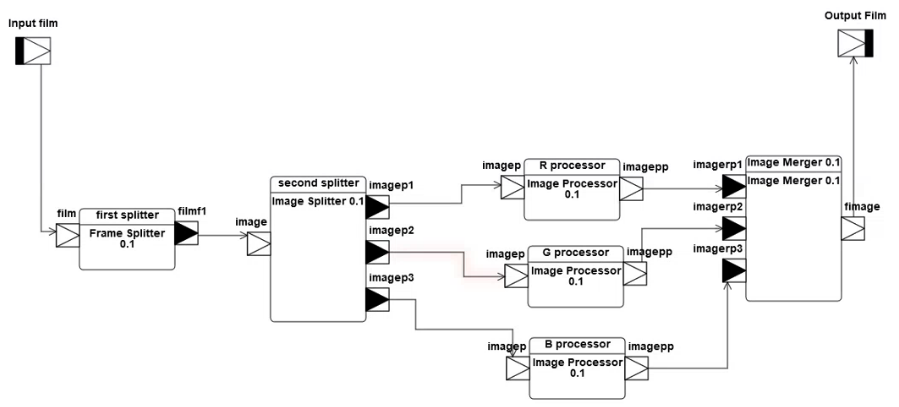
\includegraphics[width=1.0\textwidth]{images/example_app}
	\end{figure}
	
	The aim of this project is to estimate the module execution time based on input data and limited resources of the execution. The choosen approach is to create machine learning models using historical data of the module executions times.
	
	The WCET\footnote{Worst-case execution time - the maximum amout of time that the execution can take.} execution time is a crucial feature of a real-time systems\cite{wcet} when response should be guaranteed within a specified timing constraint or system should meet the specified deadline. In this project we do not strictly focus on providing an estimation of maximum execution time (WCET). We will try to estimate the average-case execution time (ACET) which is absolutely enought for this use case requirements.
	\section{Model features}
	To predict time of module execution we create a machine learning model for each module. With each execution of the module, within some application, we will get another data point to train our model. We will use the following features (explanatory variables)\footnote{As a docker container that will be used to execute a module do not use SWAP memory, RAM is not colerated with execution time. In this program we will not use modules with GPU support. Summarazing, the GPUs and RAM resources limits are not taken into account for modeling.} as an input data for the model:
	\begin{enumerate}
		\item mCPU limit - called \textit{mili cores} - the fraction of a physical CPU used to carry out the module execution,
		\item total size of an input data,
		\item max element size of an input data (if the input data is a set of files type it is the biggest part of data to be processed),
		\item avg size of an input element,
		\item number of input data elements.
	\end{enumerate}
	This last three features makes sense only if the input data is a set of files. Otherwise, if the data is just a single file (e.g. data frame), the features set should be reduced to just the first two elements from the list above.
	
	Obviously, our dependent value (that we are going to estimate) is an execution time of a module. The example data frame that will be used to train and validate our models is presented in the table~\ref{tab:example_df}.
	
	\begin{center}
		\begin{table}
			\begin{tabular}{|c c c c c c >{\columncolor[gray]{0.9}}c|} 
				\hline
				Module ID & mCPU & total [KB] & max [KB] & avg [KB] & \# & time [ms] \\ [0.5ex] 
				\hline\hline
				1 & 1.1 & 12414 & 1341 & 871 & 21 & 7813 \\ 
				\hline
				1 & 0.5 & 12414 & 1341 & 871 & 21 & 12406  \\
				\hline
				1 & 3.6 & 54001 & 2190 & 891 & 82 & 9017 \\
				\hline
				... & ... & ... & ... & ... & ... & ... \\ [1ex] 
				\hline
			\end{tabular}
		\caption{\label{tab:example_df}The example data frame for models training and validations.}
		\end{table}
	\end{center}
	\section{Algorithm}
	As a machine learning algorithm for our project we will use \textit{Epsilon-Support Vector Regression}\cite{svrc} (SVR) - it is based on Support Vector Machine (SVM, orginally named \textit{support-vector networks}\cite{svm}).
	
	We will use SVR model with a RBF kernel\cite{rbf_kernel} which is the most known flexible kernel and it could project the features vectors into infinite dimensions. It uses Taylor expansion which is equivalent to use an infinite sum over the polynomial kernels. It allows to model any function that is a sum of uknown degree polynomials.
	
	\section{Testing modules}
	
	In the project we will use the modules described below to perform models evaluations:
	
	\begin{enumerate}
		\item Face recogniser - takes set of files (images) as an input data and marks faces of people on each image.
		\item ...
	\end{enumerate}
	
	\section{Training and test datasets}

	\section{Models learning and validation}
	
	\section{Conslusions}
	
	\begin{thebibliography}{9}
		\bibitem{baltic_lsc_website} 
		BalticLSC: main webpage of the project, visited 14.03.2021,
		\\\texttt{https://www.balticlsc.eu/}
		\bibitem{baltic_lsc} 
		 BalticLSC: BalticLSC Admin Tool Technical Documentation, Design of the Computation Application Language, Design of the BalticLSC Computation Tool, visited 14.03.2021,
		\\\texttt{https://www.balticlsc.eu/wp-content/uploads \newline /2020/03/O5.2A\_O5.3A\_O5.4ABalticLSC\_Software\_Design.pdf}
		\bibitem{svm} 
		Support-Vector Networks by Corinna Cortes , Vladimir Vapnik, 1995
		\\\texttt{https://citeseerx.ist.psu.edu/viewdoc/summary?doi=10.1.1.15.9362}
		\bibitem{rbf_kernel} 
		Radial basis function kernel, Wikipedia, visited 27.12.2020
		\\\texttt{https://en.wikipedia.org/wiki/Radial\_basis\_function\_kernel}
		\bibitem{svrc} 
		Support Vector Regression, Dr. Saed Sayad, visited 17.01.2021
		\\\texttt{https://www.oreilly.com/library/view/introduction-to-machine
			/9781449369880/ch04.html}
		\bibitem{wcet} 
		Estimation of the execution time in real-time systems, 22.01.2016
		\\\texttt{https://link.springer.com/article/10.1134/S0361768816010059}
	\end{thebibliography}
	
	
\end{document}